% Marcador de pendências: tudo que aparece em vermelho precisa de dado medido ou referência a confirmar antes da entrega.
\newcommand{\pendente}[1]{\textcolor{red}{[PENDENTE: #1]}}

% Foto do protótipo final: usa images/prototype/<arquivo>.jpg (ou .png); sem o arquivo, mostra um quadro reservado.
\newcommand{\fotofinal}[3]{%
\begin{figure}[htbp]
\centering\caption{#2}\label{#3}
\IfFileExists{images/prototype/#1.jpg}{\includegraphics[width=.7\textwidth]{prototype/#1.jpg}}{%
\IfFileExists{images/prototype/#1.png}{\includegraphics[width=.7\textwidth]{prototype/#1.png}}{%
\fbox{\parbox[c][6cm][c]{.7\textwidth}{\centering\textit{Espaço reservado para a foto}\\[2pt]\texttt{\detokenize{images/prototype/#1.jpg}}}}}}
\fonte{Elaborado pelos autores (2026).}
\end{figure}}

\chapter{INTRODUÇÃO}\label{cap:introducao}

Veículos aéreos multirrotores só permanecem no ar enquanto uma malha de realimentação corrige a atitude centenas de vezes por segundo. Se a leitura do sensor, o cálculo do controle ou a atualização dos motores atrasam além do que a planta tolera, a atitude diverge e o veículo cai. Esse tipo de aplicação é o exemplo clássico de sistema de controle crítico: o resultado correto só vale se for entregue dentro do prazo \cite{burns2009,buttazzo2011}.

Este trabalho estuda esse problema em escala de bancada. A Plataforma de Estabilização Ativa por Empuxo é uma haste com um grau de liberdade (1DOF) que gira em torno de um eixo, com um motor e uma hélice em uma ponta e um sensor inercial MPU6050 na ponta oposta. O motor só empurra a haste para cima; a gravidade a puxa para baixo. O microcontrolador STM32F103 lê o ângulo, calcula o empuxo necessário e mantém a haste na horizontal, de modo análogo ao que um controlador de voo faz com um eixo de atitude de um drone. Plataformas desse tipo são usadas para estudar modelos de helicópteros e estratégias de controle \cite{cuero2020,mane2019,uyar2024}.

O objetivo da disciplina é aplicar sistemas operacionais de tempo real. Por isso, o trabalho não se limita a fazer a haste equilibrar: mostra como o FreeRTOS organiza a aplicação em tarefas, sincroniza a interrupção do temporizador com a tarefa de controle por um semáforo, protege dados compartilhados com \textit{mutexes} e isola a comunicação serial para que ela não atrase a malha crítica.

O código-fonte do firmware, os dados medidos, os \textit{scripts} de simulação e este texto estão no repositório \url{https://github.com/rickelmedias/1-DOF-Copter-Control}. O texto segue a ordem em que o projeto foi construído. O Capítulo~\ref{cap:rtos} justifica a escolha de um sistema crítico, resume o RTOS e o FreeRTOS e apresenta os fundamentos de controle usados. O Capítulo~\ref{cap:processo} traz a modelagem e a simulação. O Capítulo~\ref{cap:materiais} descreve materiais, ligações e montagem. O Capítulo~\ref{cap:desenvolvimento} detalha o firmware: módulos, configuração do STM32, tarefas e objetos do FreeRTOS, de forma que a montagem possa ser replicada. O Capítulo~\ref{cap:dificuldades} relata as dificuldades encontradas (aquecimento do motor, ruído do sensor, ajuste do PID) e as soluções. Os resultados, o refino dos ganhos do PID com testes na bancada (Capítulo~\ref{cap:refino}) e a conclusão fecham o trabalho.

\section{APRESENTAÇÃO DO GRUPO}

O trabalho é desenvolvido na disciplina Tópicos Especiais Engenharia da Computação II, do curso de Engenharia da Computação do Centro Universitário Facens, por Gustavo Aguiar Brandão (RA 210349), Lucas Carvalho (RA 180352), Rickelme Dias (RA 224276), Guilherme Cambi Magarotti (RA 222292) e Guilherme Felipe Reis Soares (RA 211590), sob orientação do Prof. Marcos F. Jardini.

\section{O PROTÓTIPO}

A estrutura é impressa em 3D: uma caixa fechada abriga parte da eletrônica (Blue Pill e driver do motor) e serve de base para a haste, que gira presa por um parafuso com porca travada, no papel de eixo. Na ponta da haste fica o motor com a hélice; na ponta oposta, o MPU6050, que mede a inclinação. Um indutor em série com o motor mantém a corrente contínua em vez de pulsada (Capítulo~\ref{cap:dificuldades}). As fotos do protótipo final estão no Capítulo~\ref{cap:materiais} (Figuras~\ref{fig:final_cima} a~\ref{fig:final_tras}). A Figura~\ref{fig:prototipo3d} mostra o modelo tridimensional inicial da haste e do suporte, anterior à caixa, e a Figura~\ref{fig:hardware} a primeira montagem eletrônica, com a Blue Pill e o módulo do driver em placa ilhada; o BEC, a chave e o indutor foram acrescentados depois (Capítulo~\ref{cap:materiais}).

\begin{figure}[htbp]
  \centering
  \caption{Modelo tridimensional inicial da haste e do suporte.}
  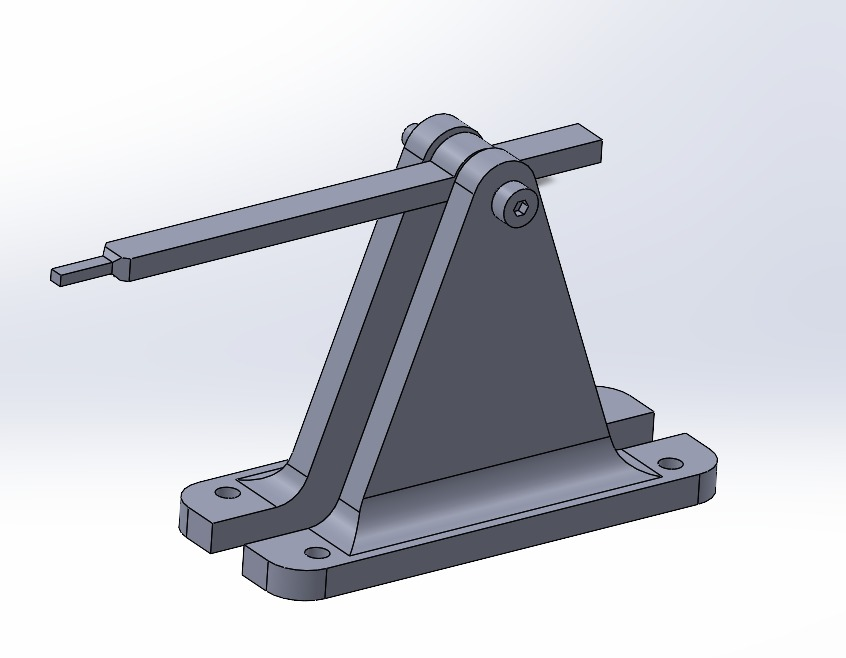
\includegraphics[width=.72\textwidth]{prototype/estrutura.jpg}
  \label{fig:prototipo3d}
  \fonte{Elaborado pelos autores (2026).}
\end{figure}

\begin{figure}[htbp]
  \centering
  \caption{Primeira montagem eletrônica: Blue Pill e driver DRV8871 em placa ilhada.}
  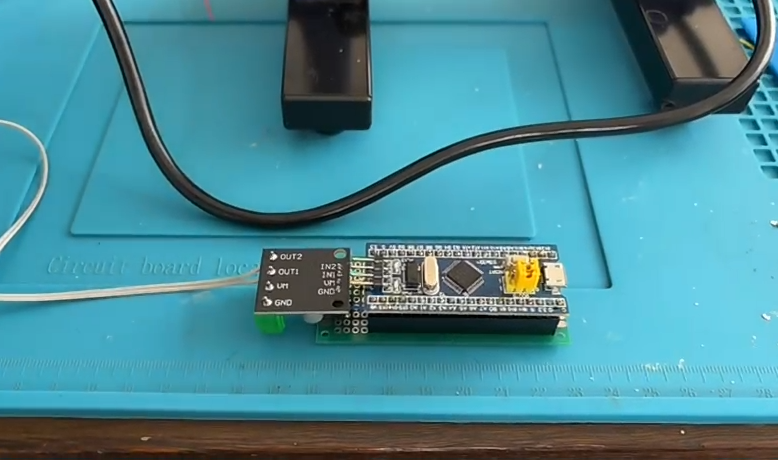
\includegraphics[width=.72\textwidth]{prototype/eletronica.png}
  \label{fig:hardware}
  \fonte{Elaborado pelos autores (2026).}
\end{figure}

\section{OBJETIVOS E ESCOPO}

O objetivo geral é projetar, construir e avaliar uma malha de estabilização angular com FreeRTOS no STM32F103, mantendo a haste próxima de $0^\circ$ e demonstrando a aplicação do RTOS a um sistema de controle crítico. Como objetivos específicos:

\begin{alineastcc}
 \item justificar a escolha de um sistema crítico e os fundamentos de RTOS e FreeRTOS que sustentam o projeto;
 \item modelar a dinâmica da haste e simulá-la para escolher e comparar controladores;
 \item montar o protótipo e documentar materiais, ligações e configuração do microcontrolador de forma replicável;
 \item organizar a malha de controle (aquisição, filtragem, PID e acionamento) em uma tarefa periódica de maior prioridade e os comandos e a telemetria em tarefas de menor prioridade, com semáforo, \textit{mutexes} e fila;
 \item tratar o ruído do MPU6050 com filtro complementar e evitar o \textit{windup} da ação integral;
 \item avaliar o equilíbrio da haste e o desempenho temporal do controle.
\end{alineastcc}

O estudo abrange um eixo de rotação e um único atuador, com referência em $0^\circ$ (horizontal). O PID foi adotado por sua estrutura simples e porque uma implementação anterior em Arduino, sem RTOS, já havia equilibrado a haste de forma qualitativa. Essa observação motivou o projeto, mas não é medida de desempenho.

\clearpage
\section{CRONOGRAMA GERAL}
A Figura~\ref{fig:cronograma} apresenta o cronograma de Gantt elaborado pelo grupo para o período de agosto a dezembro de 2026. A imagem reúne as atividades, suas durações e os marcos de entrega previstos.
\begin{figure}[H]
\centering
\caption{Cronograma de Gantt do projeto.}\label{fig:cronograma}
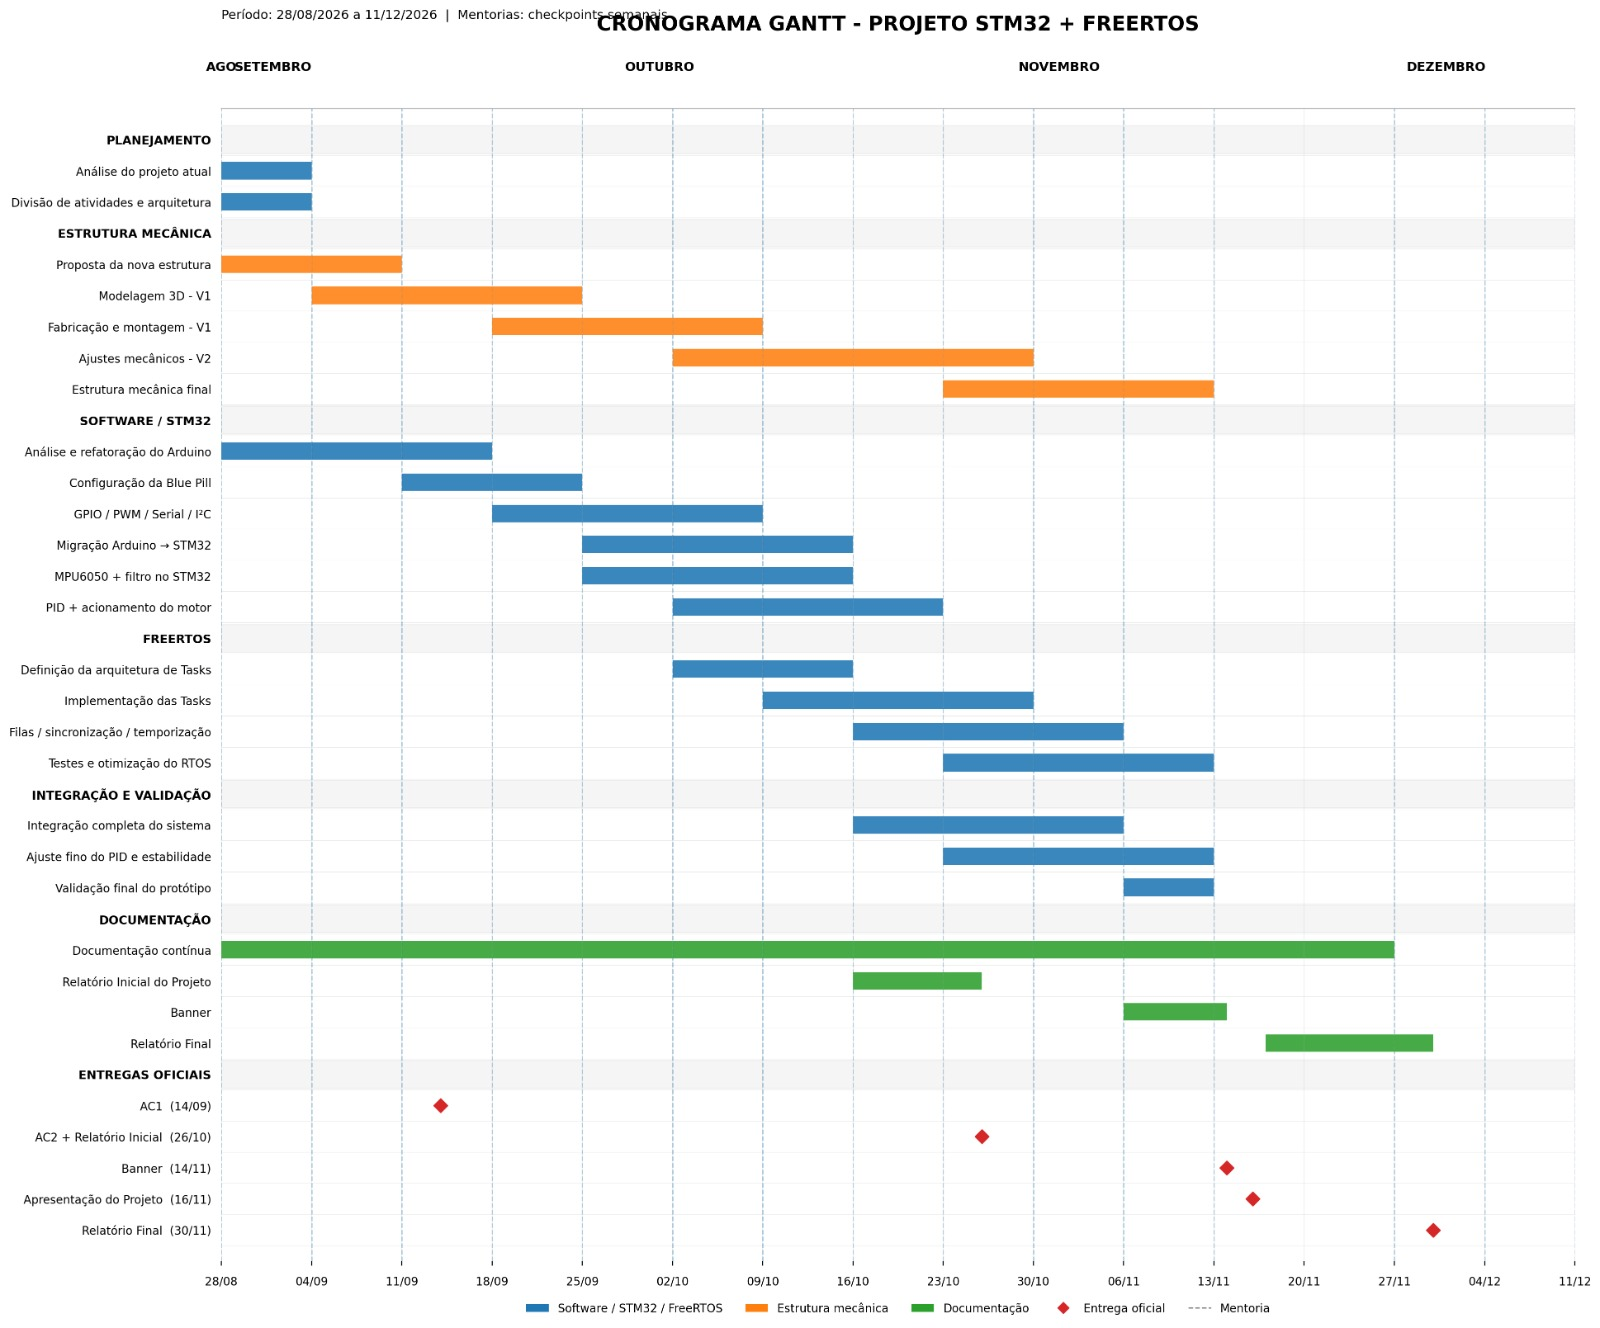
\includegraphics[width=\textwidth]{cronograma-gantt.jpg}
\fonte{Elaborado pelos autores (2026).}
\end{figure}
